\graphicspath{{./chapters/04/assets/}}
\chapter{Secondo Progetto}
Il secondo progetto assegnatomi durante il periodo di tirocinio mi ha permesso di approfondire ancora di più le tecnologie trattate nel Capitolo~\ref{cha:analisiTecnologie} e di utilizzare le competenze di programmazione apprese durante il percorso di Laurea, sviluppando dei Plugin in linguaggio C\#. 

La motivazione che ha spinto il supervisore aziendale ad affidarmi questo progetto risiede nel fatto che l'azienda necessitava di una \textit{demo proof-of-concept} da utilizzare come esempio delle possibilità di customizzazione del CRM per i potenziali clienti. Il progetto sviluppato infatti modella un processo di business\footnote{Anche se semplificato.} per le società che operano nel settore della fornitura energetica per aziende. 

Lo scenario fittizio che il tutor aziendale, insieme all'analista funzionale, ha progettato per me è quello di un'azienda che offre forniture di energia elettrica e gas per aziende.
Vista l'alta mole di lavoro, tale società necessita di un sistema che permetta di velocizzare e rendere più efficiente il processo di creazione di preventivi e offerte personalizzate per i propri clienti e quindi ha commissionato la soluzione di questo problema a Cluster Reply.

\section{Processo di business}
Il processo di business che mi è stato chiesto di modellare consiste nella gestione semi-automatica di una richiesta di fornitura di energia personalizzata per una azienda cliente, basata sul processo standard del CRM Lead-Opportunity-Quote-Order del modulo funzionale Sales e sui Case del modulo funzionale Service.
In Figura~\ref{fig:processoUtilities} un diagramma del processo modellato. 

\begin{figure}[ht]
  \centering
  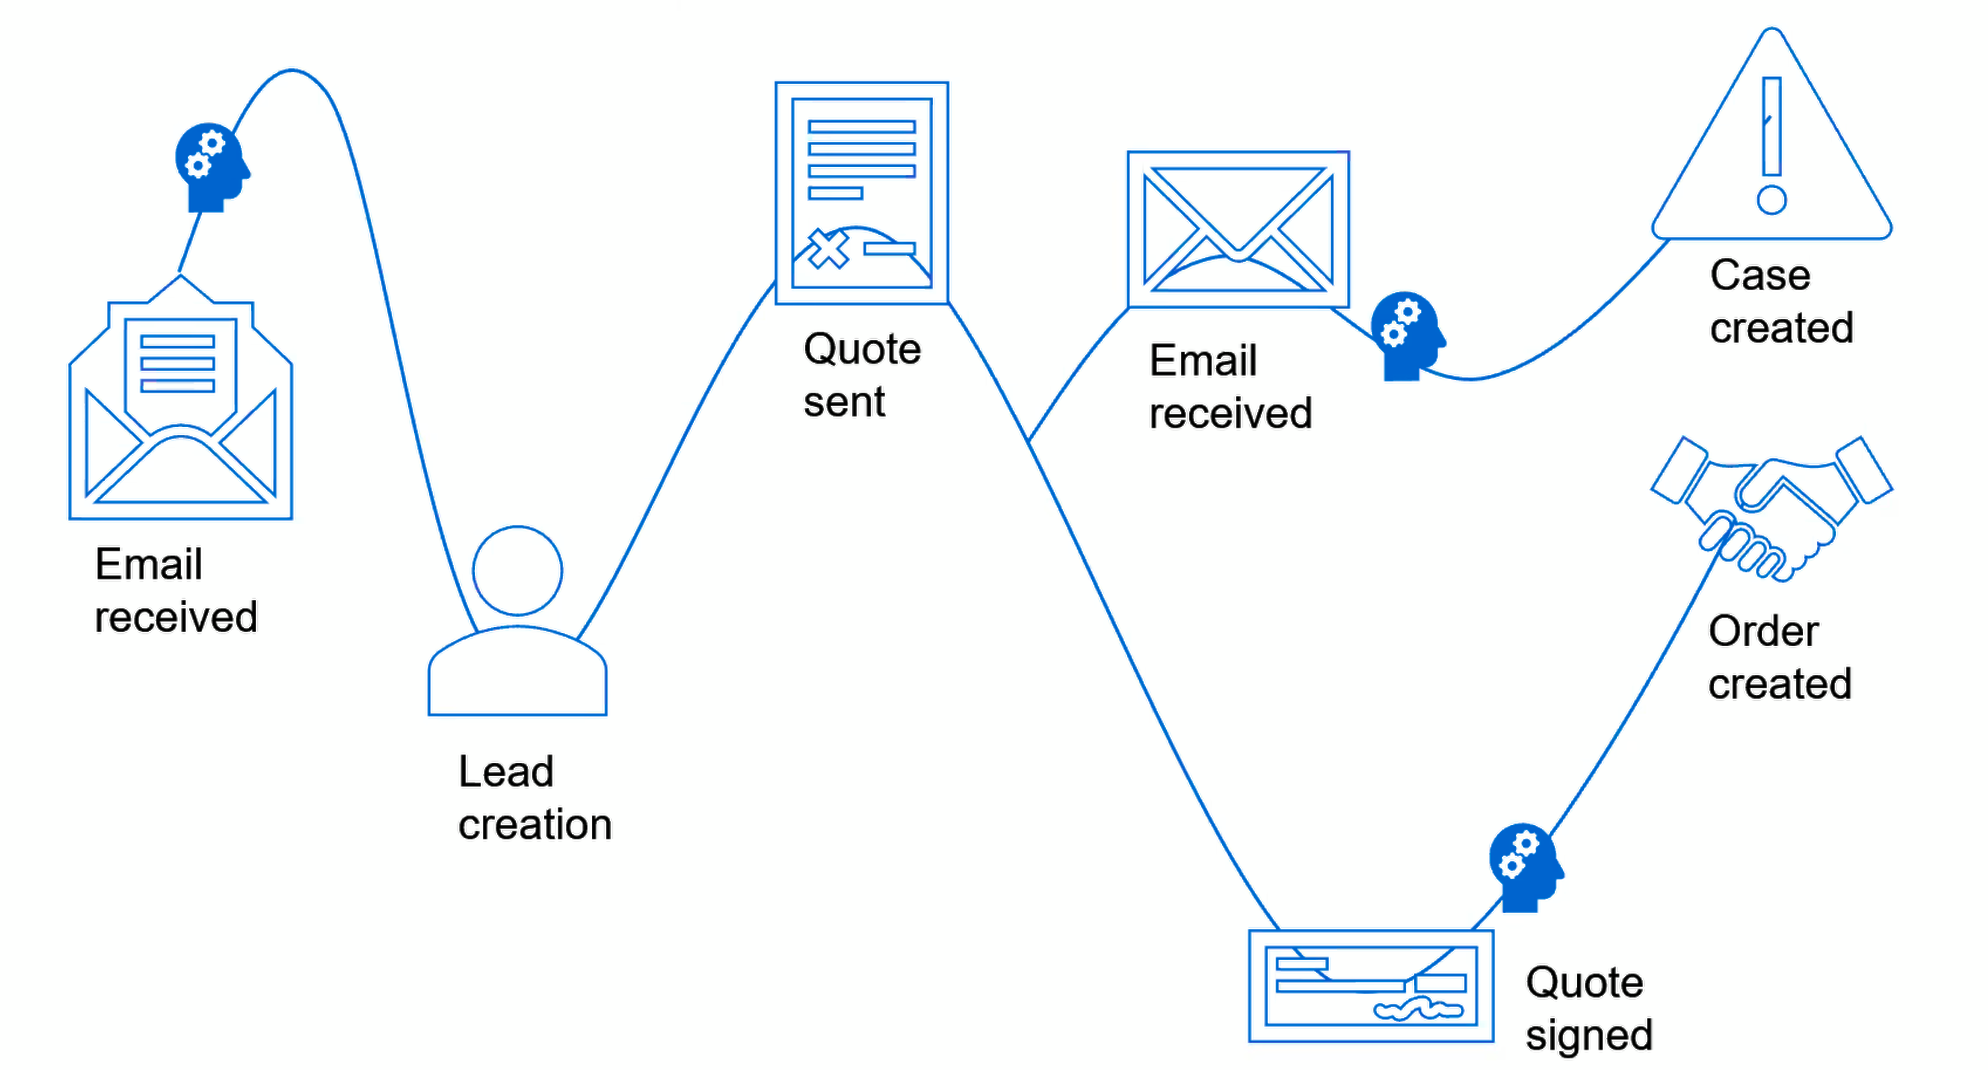
\includegraphics[width=0.8\textwidth]{processo-utilities.png}
  \caption{Processo di business modellato dal progetto.}
  \label{fig:processoUtilities}
\end{figure}

Nel dettaglio si compone dei seguenti passaggi:
\begin{enumerate}
  \item Arrivo di un'email da parte di un potenziale cliente con in allegato un modulo compilato. Il modulo contiene informazioni riguardanti il cliente stesso (anagrafica) e le necessità di fornitura di energia per le quali ha effettuato la richiesta di preventivo.
  \item Il documento viene processato automaticamente mediante AI Builder e viene creato un nuovo record Lead nel CRM. Nel caso in cui il documento non venga processato correttamente o si verifichino errori viene inviata un'email di cortesia al potenziale cliente che notifichi l'errore.
  \item In seguito alla creazione del Lead quest'ultimo viene automaticamente \textit{qualificato} in un record Opportunity mediante un Plugin.
  \item Un operatore compila manualmente il preventivo (Quote) di fornitura basandosi sui dati raccolti in precedenza. 
  \item  Quando il preventivo viene contrassegnato come ''attivo'', viene avviato un secondo plugin che invia automaticamente un'email al cliente contenente il preventivo come allegato.
  \item 
  \begin{itemize}
    \item Se il cliente risponde all'email con il preventivo firmato (con il controllo effettuato automaticamente grazie a un modello AI Builder), il Quote si considera vinto e viene convertito in Order per poi essere ultimato da un operatore. 
    \item Se il cliente risponde all'email in qualsiasi altro modo, un modello di classificazione di categoria di AI Builder analizza il testo dell'email. Sulla base dell'output di questo modello, viene creato un record Case e assegnato a un'apposita coda del modulo funzionale Service per essere processato da un operatore.
  \end{itemize}
\end{enumerate}

\section{Sviluppo del progetto}
In seguito alla definizione dettagliata dei requisiti ho proceduto con lo sviluppo del progetto che ha richiesto l'utilizzo di Power Automate, AI Builder, Plugin e customizzazioni di form e regole di \textit{routing} per l'instradamento dei Case nelle varie Queue.

\subsection{AI Builder}
Sono stati utilizzati due diversi tipi di modelli AI Builder:
\begin{itemize}
  \item Modello personalizzato per l'elaborazione di moduli - utilizzato per l'estrazione di dati dal modulo di richiesta preventivo e per verificare l'accettazione del preventivo.
  \item Modello predefinito di classificazione delle categorie per classificare il contenuto dell'email di risposta all'invio del preventivo.
\end{itemize}

\subsubsection{Modulo di richiesta preventivo}
Avendo praticamente carta bianca su come sviluppare il modulo ho potuto evitare le problematiche riscontrate durante il primo progetto. In Figura~\ref{fig:moduloRichiestaPreventivo} un esempio di modulo. Per questo progetto, come indicato dal mio supervisore, non mi sono soffermato in modo eccessivo sul training del modello e ho utilizzato semplicemente un campione di \num{5} documenti compilati. Per brevità, inoltre, non riporto l'elenco dei campi riconosciuti, in quanto corrispondono alle celle compilabili del documento in Figura~\vref{fig:moduloRichiestaPreventivo}.

\begin{figure}[ht!]
  \centering
    \subfloat[][\emph{Pagina 1.}]
       {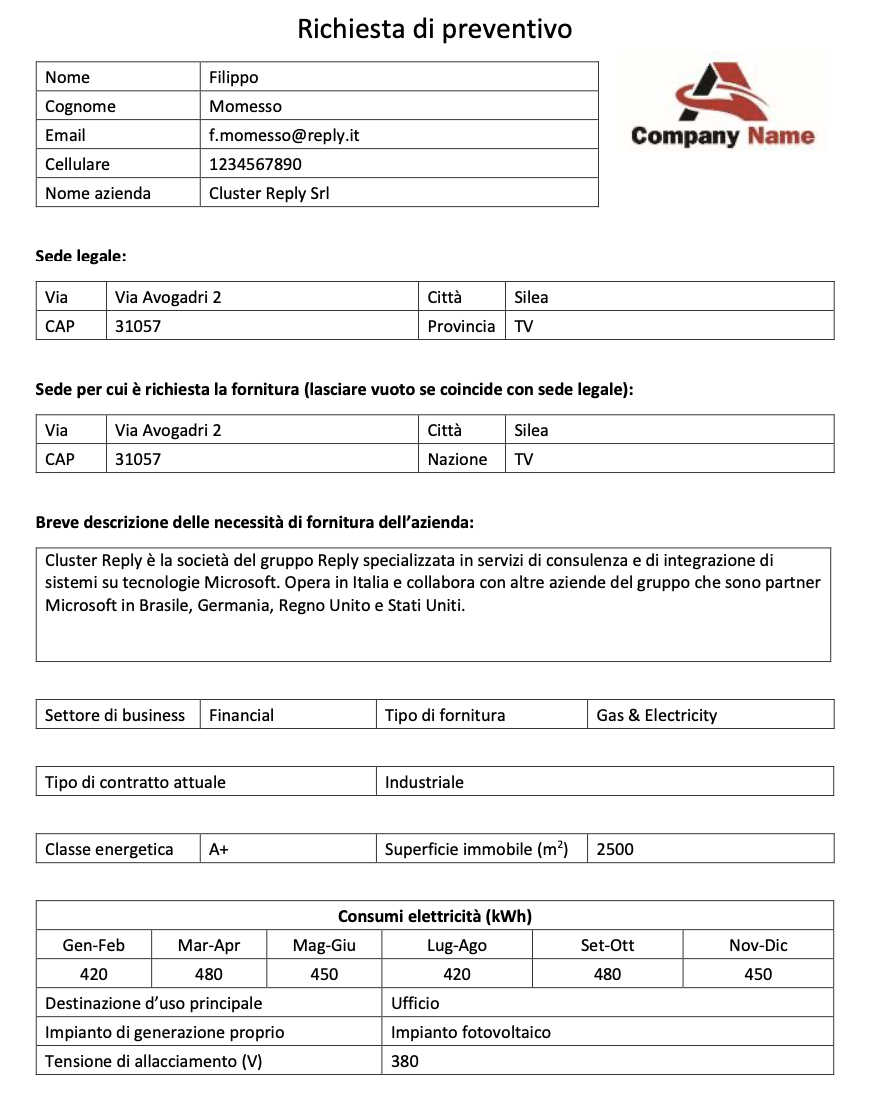
\includegraphics[width=.45\textwidth,valign=c]{modulo-richiesta-preventivo1.png}} \quad
    \subfloat[][\emph{Pagina 2.}]
       {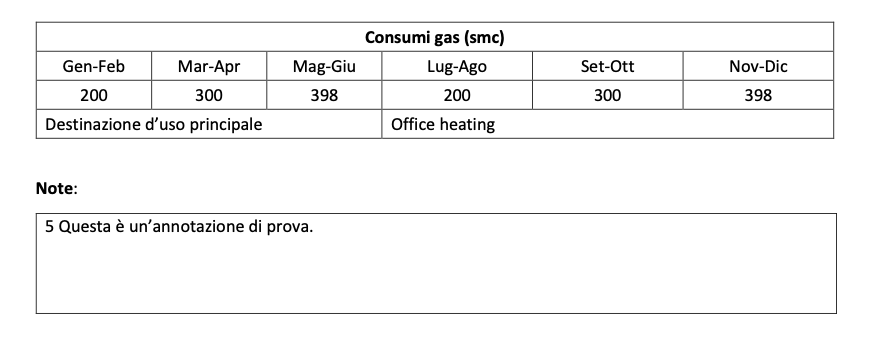
\includegraphics[width=.45\textwidth,valign=c]{modulo-richiesta-preventivo2.png}} \\
  \caption{Esempio di modulo utilizzato.}
  \label{fig:moduloRichiestaPreventivo}
\end{figure}

\subsubsection{Documento con preventivo accettato}
Per l'accettazione del preventivo si è optato per l'apposizione di data e firma. È stato dunque creato un modello di elaborazione di moduli che rilevasse nome del cliente, ID del Quote, data e firma. Tuttavia, come riportatato in Sezione~\ref{ssec:creazioneModello}, il rilevamento di firme non è ancora supportato da AI Builder ma stando a informazioni interne giunte a Cluster Reply, lo sarà in futuro. Pertanto, in fase di validazione del documento, la firma verrà semplicemente ignorata e i controlli verranno effettuati solamente sui restanti campi analizzati. In Figura~\ref{fig:documentoPreventivo} un esempio di documento utilizzato per questo modello. Anche in questo caso per il training è stato utilizzato un campione di \num{5} documenti compilati.

\begin{figure}[ht!]
  \centering
  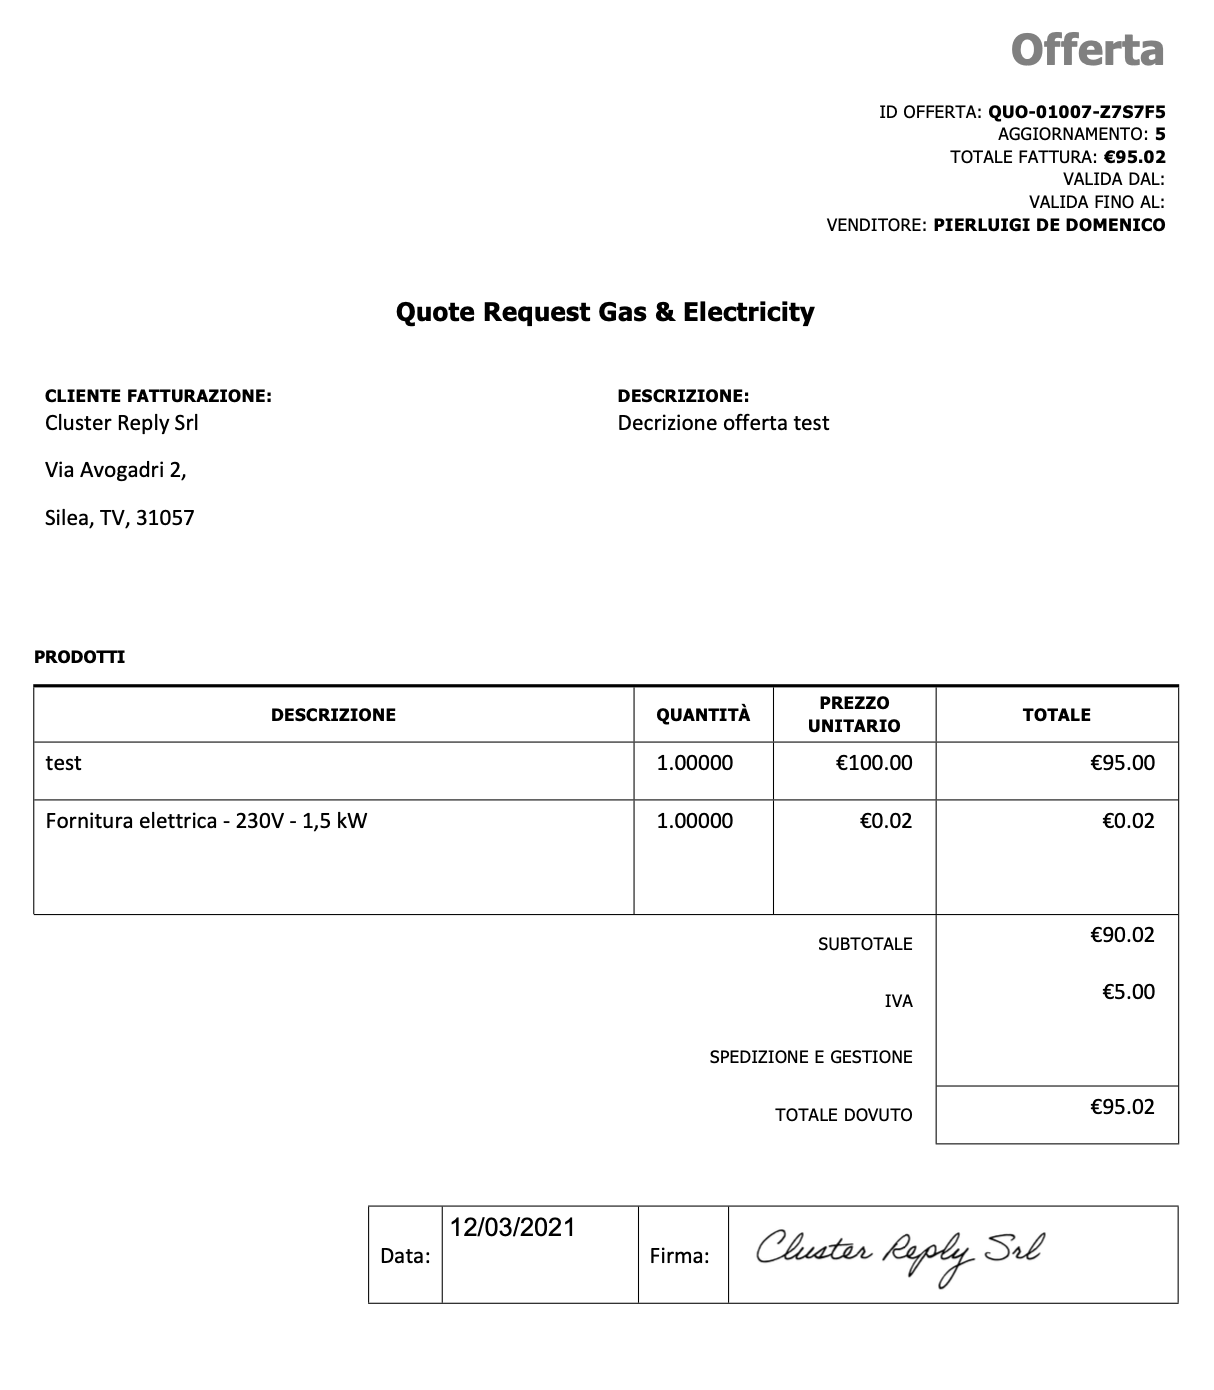
\includegraphics[width=0.5\textwidth]{documento-preventivo.png}
  \caption{Esempio di preventivo compilato e firmato per accettazione.}
  \label{fig:documentoPreventivo}
\end{figure}

\subsection{Flussi Power Automate}
Sono stati sviluppati due flussi cloud: il primo copre le fasi del processo che vanno dalla ricezione dell'email con allegato fino alla creazione del Lead; il secondo, invece, si occupa di gestire quanto avviene dopo l'invio del preventivo, ovvero la risposta positiva o negativa del cliente.

\subsubsection{Flusso di creazione del Lead}
In Figura~\ref{fig:flussoCreazioneLead} è riportato il primo flusso cloud sviluppato, il quale si occupa di creare il Lead a partire dai dati estratti dal documento ricevuto come allegato dell'email.

Si compone di diverse fasi:
\begin{enumerate}
  \item Trigger sulla creazione di un record Attachment.
  \item Controlli su destinatario dell'email e tipo di documento.
  \item Conversione del documento in PDF se l'allegato non è in formato PDF.
  \item Estrazione dei dati dal documento mediante modello AI Builder.
  \item Operazioni di validazione sui dati estratti
  \item Creazione del Lead e aggiornamento del campo Regarding dell'email in modo da associarla al Lead.
\end{enumerate}

\begin{figure}[ht!]
  \centering
  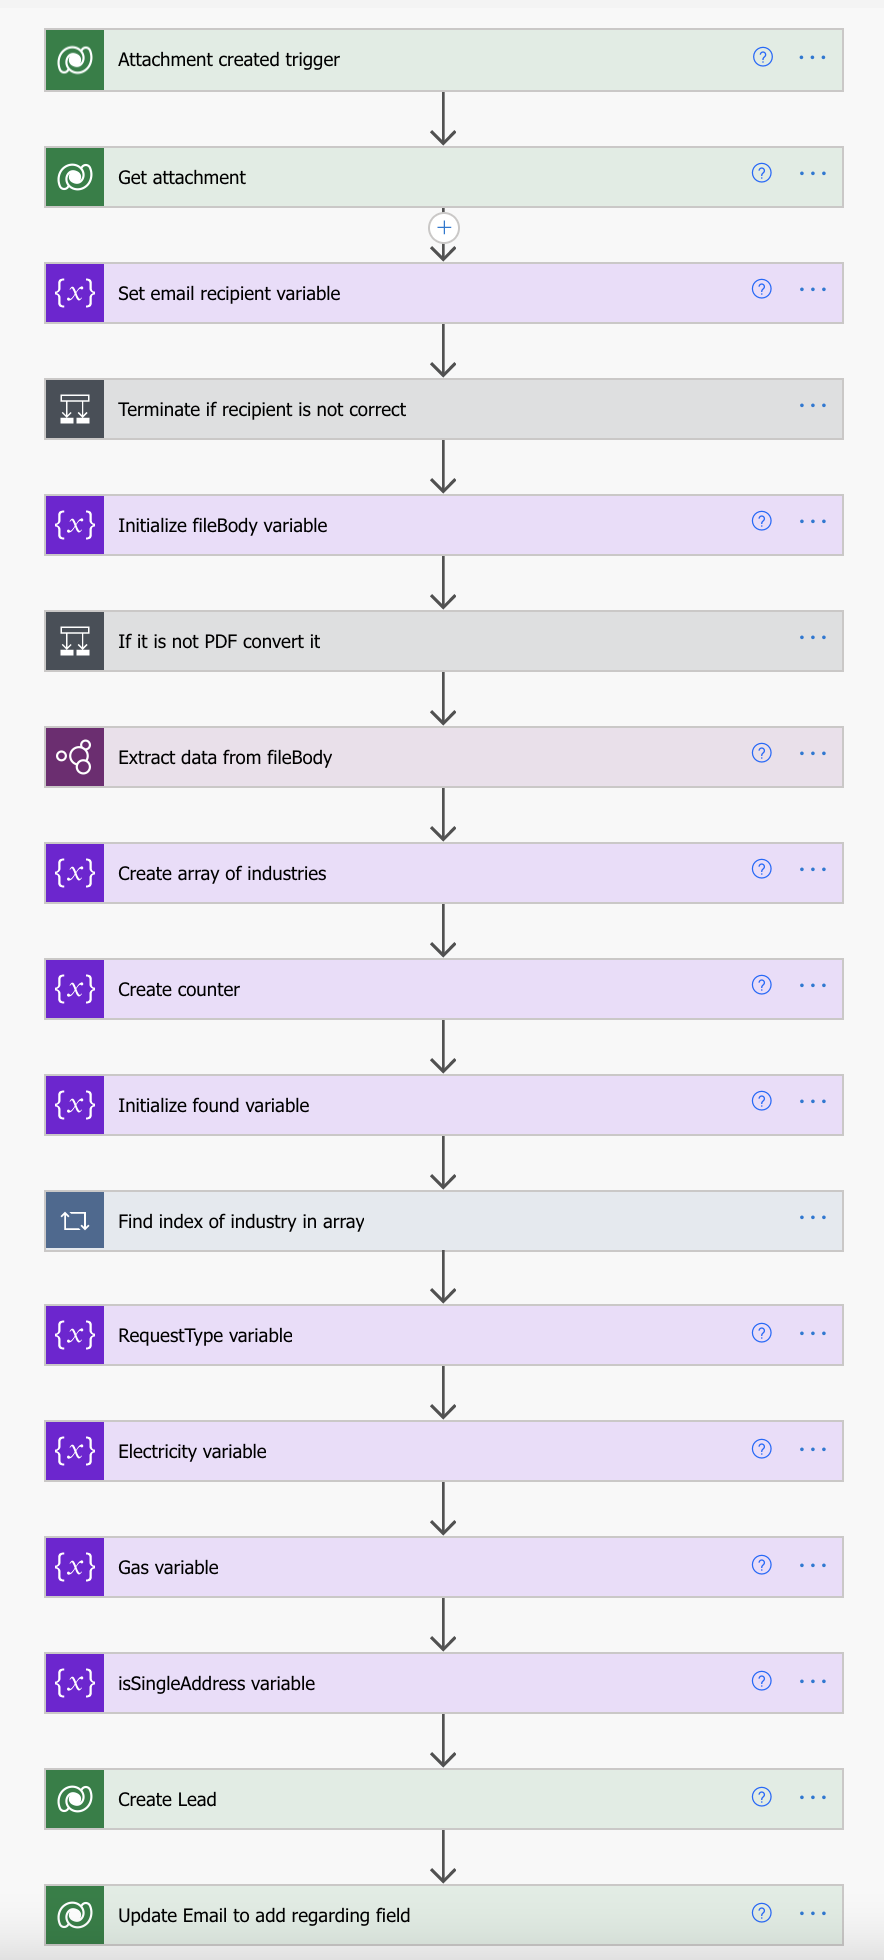
\includegraphics[width=0.45\textwidth]{flusso1.png}
  \caption{Flusso di creazione del Lead}
  \label{fig:flussoCreazioneLead}
\end{figure}

\subsubsection{Flusso di elaborazione della risposta del cliente}
Il flusso che viene eseguito in seguito alla ricezione di un'email di risposta a un preventivo è più articolato in quanto necessita di gestire due possibilità: offerta accettata oppure offerta rifiutata.

Si compone delle seguenti fasi:
\begin{enumerate}
  \item Trigger sulla creazione di un record Email e controllo che l'email sia associata ad un record Quote. Il CRM si occupa in automatico di creare le relazioni se un'email viene ricevuta come risposta ad un'email associata ad un record mediante il campo Regarding.
  \item Recupero di un eventuale allegato. Se presente il processo procede con:
  \begin{enumerate}
    \item Conversione del documento in formato PDF se non è in formato PDF.
    \item Estrazione dei dati dal documento mediante modello AI Builder.
    \item Validazione sui dati estratti con controllo sulle confidence. Un valore medio di confidence sui valori riconosciuti inferiore a \num{0.7} rende non valido il documento.
    \item Se il documento è valido e firmato, il Quote è considerato vinto e pertanto convertito in Ordine.
  \end{enumerate}
  \item Se il documento non è presente o risulta non valido, segue l'analisi del testo dell'email mediante il modello di classificazione di categorie.
  \item Creazione del Case il cui campo Description contiene l'output del modello utilizzato nella fase precedente e aggiornamento del campo Regarding dell'email in maniera tale da associarla al Case appena creato.
\end{enumerate}

\subsection{Plugin}
Sono stati sviluppati due Plugin che svolgono le seguenti operazioni: 
\begin{itemize}
  \item Conversione del Lead in Opportunity.
  \item Invio automatico di email con preventivo in allegato.
\end{itemize}

Come strumenti di sviluppo ho utilizzato Microsoft Visual Studio unitamente a Microsoft XRM Toolbox, utile per il debugging e la registrazione dei plugin nella soluzione del CRM.

\subsubsection{Conversione del Lead in Opportunity}
\label{ssec:conversioneLead}
Per la conversione del Lead in Opportunity ho scelto di utilizzare un Plugin registrato sul Create Message in fase Post-operation dell'entità Lead. In questo modo la sua esecuzione viene avviata al termine della creazione del Lead.

Mediante un'istanza di \lstinline[language={[Sharp]C}]{IOrganizationService} si ottiene il contesto in cui il plugin viene eseguito, e in questo modo è possibile, ad esempio, avere informazioni sul record che ha avviato l'esecuzione. La classe \lstinline[language={[Sharp]C}]{ITracingService} permette di stampare dei log sul CRM. 

Per prima cosa il codice effettua dei controlli sull'esistenza di un Account o Contact a cui associare l'Opportunity una volta convertita in Lead. Con la classe \lstinline[language={[Sharp]C}]{QueryExpression} è possibile, infatti, interrogare il CRM per ottenere dei record, come fosse una SELECT su un database. Nel Listato~\ref{QueryExpressionListing} un esempio di utilizzo.

\begin{lstlisting}[language={[Sharp]C},breaklines=true,caption={Esempio di utilizzo di una QueryExpression.},label=QueryExpressionListing]
  // Check if the account already exist 
  QueryExpression accountQuery = new QueryExpression("account");
  accountQuery.NoLock = true;
  accountQuery.ColumnSet = new ColumnSet("accountid");
  accountQuery.Criteria.AddCondition(new ConditionExpression("name", ConditionOperator.Like, companyName));
  if (partitaIva != null) accountQuery.Criteria.AddCondition(new ConditionExpression("accountnumber", ConditionOperator.Like, partitaIva));
  accountQuery.PageInfo.ReturnTotalRecordCount = true;
  EntityCollection resultsAccount = service.RetrieveMultiple(accountQuery);
\end{lstlisting}

Successivamente viene utilizzato un Message \lstinline[language={[Sharp]C}]{QualifyLeadRequest}, che fornisce la funzionalità standard di conversione di un Lead in Opportunity. A quest'ultimo vengono passati come parametri il Lead da qualificare ed eventuali riferimenti a Contact o Account se già esistenti a sistema. \lstinline[language={[Sharp]C}]{QualifyLeadRequest}, infatti, si occupa di default di creare Contact e Account per il potenziale cliente a partire dal Lead e, per evitare problemi con possibili duplicati, ho deciso di disabilitare il controllo automatico e gestire i duplicati manualmente. Il Listato~\ref{QualifyLeadRequestListing} riporta quanto appena spiegato.

Altre operazioni svolte sono l'aggiornamento di alcuni campi dell'Opportunity creatasi dopo l'esecuzione del suddetto Message.

\begin{lstlisting}[language={[Sharp]C},breaklines=true,caption={Utilizzo del Message QualifyLeadRequest.},label=QualifyLeadRequestListing]
  QualifyLeadRequest qualify = new QualifyLeadRequest {
    CreateOpportunity = true,
    OpportunityCurrencyId = currencyId,
    LeadId = new EntityReference(entity.LogicalName, entity.Id),
    Status = new OptionSetValue(OptionSet.Lead.StatusCode.Qualified)
  };

  if (contactExists && !accountExists) {
    // Create account and use existing contact as OpportunityCustomerId
    qualify.CreateAccount = true;
    qualify.OpportunityCustomerId = new EntityReference("contact", contactId);
  } else if (!contactExists && accountExists) {
    // Create contact and use existing account as OpportunityCustomerId
    qualify.CreateContact = true;
    qualify.OpportunityCustomerId = new EntityReference("account", accountId);
  } else if (contactExists && accountExists) {
    // Use existing account as OpportunityCustomerId
    qualify.OpportunityCustomerId = new EntityReference("account", accountId);
    //if contact is not associated to account 
  } else {
    qualify.CreateAccount = true;
    qualify.CreateContact = true;
  }

  //Disable DuplicateDetection
  qualify.Parameters.Add("SuppressDuplicateDetection", true);

  QualifyLeadResponse qualifyRes = (QualifyLeadResponse)service.Execute(qualify);
\end{lstlisting}

\subsubsection{Invio di email con preventivo}
\label{ssec:invioEmail}
Per l'invio automatico dell'email con il preventivo, ho deciso di utilizzare un Plugin registrato sull'Update Message in fase Post-operation dell'entità Quote. 

Per prima cosa viene controllato che il campo \textit{statecode} sia stato aggiornato ad \textit{attivo}, altrimenti l'esecuzione viene interrotta.
Dopodiché viene generato il documento PDF con il preventivo, codificato in formato \textit{base64}, mediante una chiamata all'Organization Web Service, come visibile nel Listato~\ref{OrganizationRequestListing}.

\begin{lstlisting}[language={[Sharp]C},breaklines=true,label=OrganizationRequestListing,caption=Chiamata all'azione ExportPdfDocument per la creazione del documento PDF.]
  private String generateEncodedPdf(IOrganizationService service, Entity quote, Guid documentTemplateId) {
      // Request to create pdf
      OrganizationRequest createPdfRequest = new OrganizationRequest("ExportPdfDocument");
      createPdfRequest["EntityTypeCode"] = 1084; // Quote typecode
      createPdfRequest["SelectedTemplate"] = new EntityReference("documenttemplate", documentTemplateId);
      createPdfRequest["SelectedRecords"] = "[\"{" + quote.Id.ToString() + "}\"]";

      OrganizationResponse createPdfResponse = (OrganizationResponse)service.Execute(createPdfRequest);

      return Convert.ToBase64String((byte[])createPdfResponse["PdfFile"]);
    }
\end{lstlisting}

Viene quindi creata l'email a partire da un template presente sul CRM. Per fare ciò prima si recupera il template attraverso una \lstinline[language={[Sharp]C}]{QueryExpression} e, successivamente, il template viene istanziato in un'email grazie a una chiamata al Message \lstinline[language={[Sharp]C}]{IstantiateTemplateRequest}. Nel Listato~\ref{GenerateEmailFromTemplate} è consultabile il codice corrispondente.
L'email viene poi completata con i valori \textit{destinatario} e \textit{mittente} e vien quindi creato un record Attachment sul CRM utilizzando il documento in formato \textit{base64} generato in precedenza.
Infine, l'email viene inviata mediante un Message \lstinline[language={[Sharp]C}]{SendEmailRequest}.

\begin{lstlisting}[language={[Sharp]C},breaklines=true,label=GenerateEmailFromTemplate,caption={Metodo per la creazione di un'email a partire da un template.}]
    //Create a query expression to get necessary email quote template
    QueryExpression queryBuildInTemplates = new QueryExpression {
      EntityName = "template",
      ColumnSet = new ColumnSet("templateid", "title"),
      Criteria = new FilterExpression()
    };
    queryBuildInTemplates.Criteria.AddCondition("title", ConditionOperator.Equal, "Template Offerta Email");
    EntityCollection templateEntityCollection = service.RetrieveMultiple(queryBuildInTemplates);

    Guid emailTemplateId = new Guid();

    if (templateEntityCollection.Entities.Count > 0) {
      emailTemplateId = (Guid)templateEntityCollection.Entities[0].Attributes["templateid"];
    } else {
      throw new ArgumentException("Standard Email Templates are missing");
    }

    // Create the request
    InstantiateTemplateRequest emailUsingTemplateReq = new InstantiateTemplateRequest {
      // Use a built-in Email Template of type "quote".
      TemplateId = emailTemplateId,

      // The regarding Id is required, and must be of the same type as the Email Template.
      ObjectId = quote.Id,
      ObjectType = "quote"
    };

    InstantiateTemplateResponse emailUsingTemplateResp = (InstantiateTemplateResponse)service.Execute(emailUsingTemplateReq);
\end{lstlisting}

\subsection{Gestione del Case}
Nell'eventualità che il flusso di elaborazione della risposta del cliente rilevi un documento non valido oppure non presente, procede con la creazione di un record Case la cui descrizione contiene l'output del modello di classificazione di categorie.
Le categorie possibili sono le seguenti:
\begin{itemize}
  \item Issues
  \item Customer Service
  \item Documentation
  \item Price \& Billing
  \item Compliment
  \item Staff
\end{itemize}

Per facilitare la gestione dei Case da parte degli addetti del settore Service ho creato quattro Queue, in cui i Case vengono distribuiti grazie a delle \textit{routing rules} (in italiano \textit{regole di instradamento}), una funzionalità del CRM che permette di redistribuire automaticamente i record in Queue sulla base di regole appositamente definite. In Tabella~\ref{table:routingRules} è possibile osservare come ho scelto di distribuire le sei tipologie di Case nelle rispettive Queue.

\begin{table}[ht]
  \centering
  \begin{tabular}{ll}
    \toprule
      \textbf{Tipologia di Case} & \textbf{Queue} \\ 
    \midrule
    Issues & \multirow{2}*{Problemi} \\
    Customer Service &  \\
    \midrule
    Documentation & Documentazione \\
    \midrule
    Price \& Billing & Prezzo e Fatturazione \\
    \midrule
    Compliment & \multirow{2}*{Generale} \\
    Staff &  \\
    \bottomrule
  \end{tabular}
  \caption{Tipi di Web Resource supportati}
  \label{table:routingRules}
\end{table}

\section{Considerazioni sul progetto}
Diversamente dal precedente, mi ritengo soddisfatto dell'esito di questo progetto. Salvo qualche intoppo durante lo sviluppo, risolto grazie all'aiuto dei colleghi più esperti, sono riuscito a portare a termine quanto richiesto e ho ottenuto un feedback positivo da parte del mio supervisore aziendale sul lavoro svolto. Quest'ultimo, inoltre, mi ha fatto sapere che, vista la qualità del risultato, sarebbe stato realmente utilizzato come \textit{demo} da mostrare ai potenziali clienti di Cluster Reply.


